\title{Anomaly Detection in Energy Consumption} %\newline Preliminary Report}
\author{
	\hspace{5cm}  Ioannis Iossifidis \hspace{5cm}                      \\ \newline
	\and \newline
        Muhammad Ayaz Hussain \\
               \and
        Muhammad Saif-ur-Rehman\\}
\date{\today}

\documentclass[12pt]{article}
\usepackage{graphicx}
\usepackage{amsmath,amssymb}
\usepackage{afterpage}
\usepackage{float}
\usepackage{longtable}
\usepackage{ltxtable}

\begin{document}
\maketitle

%\begin{abstract}
%This is the paper's abstract and must be filled with energy concerns happening to companies these days etc etc \ldots
%\end{abstract}

\section{Problem Description}
In modern days, the amount of energy consumption is becoming a more serious issue as several companies and industries are addressing this issue in order to contain their expenses as unexpected variations can incur operational costs to their facilities. These fluctuations in electricity consumption can arise from various factors such as excessive use of heavy equipment like electric heaters in winters, room coolers during the summers etc. In order to detect such variations or anomalies, anomaly detector algorithm is designed and implemented on the provided data.


\section{Data Analysis}
\label{Data}
Initially, the raw data was provided by the Tengelmann Group, which consisted of 3 features which were timestamp, store number, and corresponding power consumption by that store during that timestamp. 
Those entries were obtained from the energy consumption data of 227 stores operated by Tengelmann Group on the hourly basis for 11 months as shown in the form of a scatter plot in Figure \ref{100blockdiag}. Analysis of which shows that there is an obvious increase in power consumption during the winter months possibly due to the usage of electric heaters also a sharp drop in the power consumption around Christmas and New Year (just above January) can be observed which indicates lower activity of those stores during that particular period of time, which makes a perfect sense and lower activity directly corresponds to lower power consumption.

\begin{figure}[H]
	\centering
	{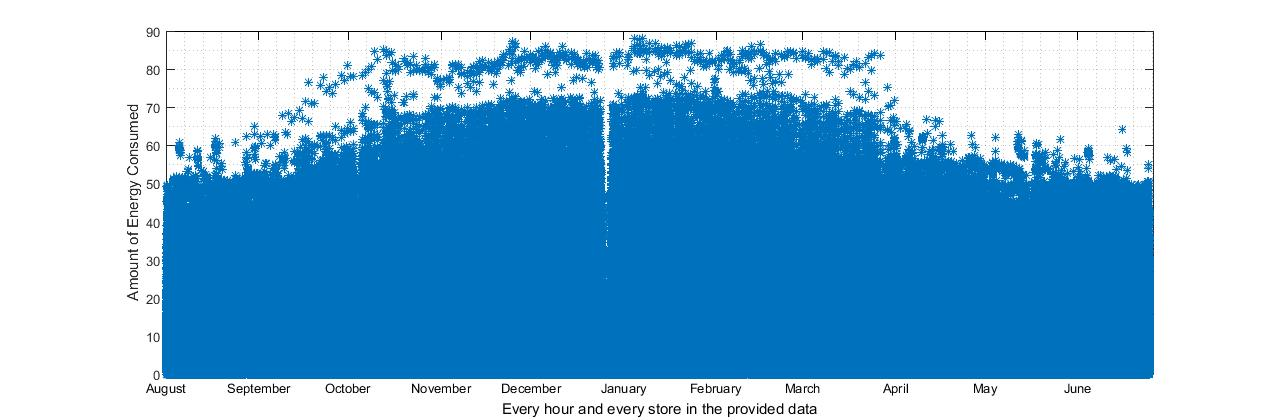
\includegraphics[scale=0.33]{All_year.jpg}\label{100blockdiag}
	}
	\caption[The Block Diagram of the designed application]{Energy Consumption by all stores during the whole time period}
	\label{100blockdiag}
	\hspace{0.7cm}%
\end{figure}
 

\paragraph{}Afterward, a random month is selected from the whole time period (in this case January 2016) and energy consumption of all stores is plotted as shown in Figure \ref{0blockdiag}.

\begin{figure}[H]
	\centering
	{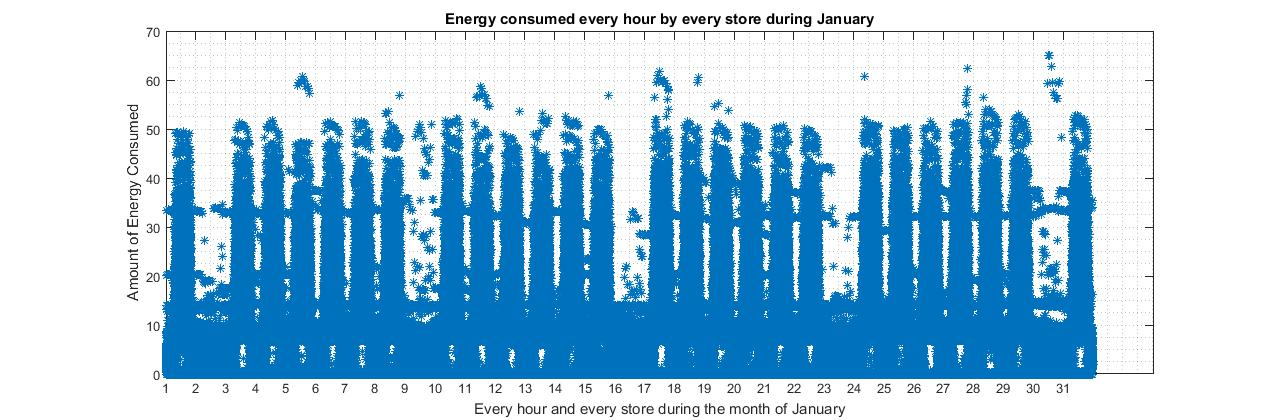
\includegraphics[scale=0.33]{Energy_alldays_allstores_jan.jpg}\label{0blockdiag}
	}
	\caption[The Block Diagram of the designed application]{Energy Consumption by all stores during January 2016}
	\label{0blockdiag}
	\hspace{0cm}%
\end{figure}

\paragraph{}Analysis of Figure \ref{0blockdiag} shows a consistent cycle of working and non working days (6 days working and one day off), which makes sense as stores remain closed on Sundays. Therefore, we added the day tag whether the particular day is a working day or a public holiday in our feature vector. 

\paragraph{}Still, it was difficult to pin point or visualize any single store from that plot. Therefore, a random store was chosen (store 105) for deeper analysis as shown in Figure \ref{101blockdiag}.

\begin{figure}[H]
	\centering
	{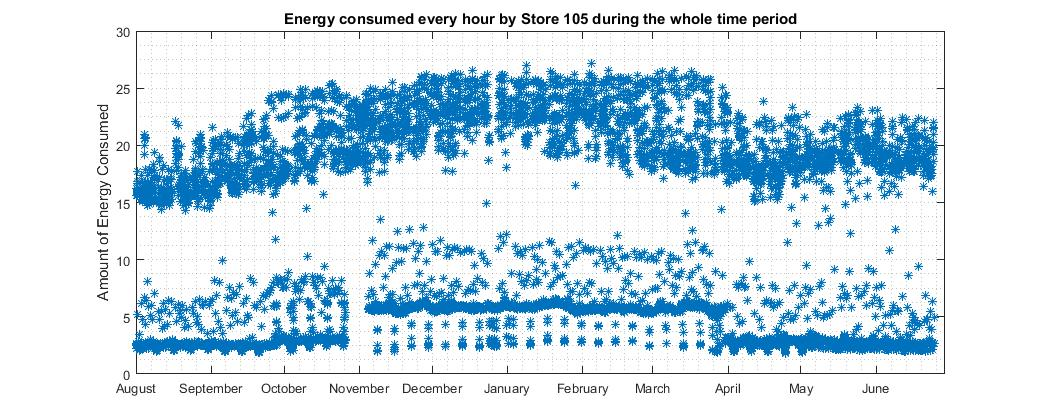
\includegraphics[scale=0.37]{new_105_jan_whole_year.jpg}\label{101blockdiag}
	}
	\caption[The Block Diagram of the designed application]{Energy Consumption by Store 105 during the whole time period}
	\label{101blockdiag}
	\hspace{0.7cm}%
\end{figure}

\paragraph{}We can again see the noticeable increase in  energy consumption during winter months from October to April as well as lower consumption during Christmas and New year holidays. 


\paragraph{}Again, we have used the month of January which was randomly picked earlier in order to visualize the energy consumption by store 105 during that month which is shown in Figure \ref{102blockdiag}.

\begin{figure}[H]
	\centering
	{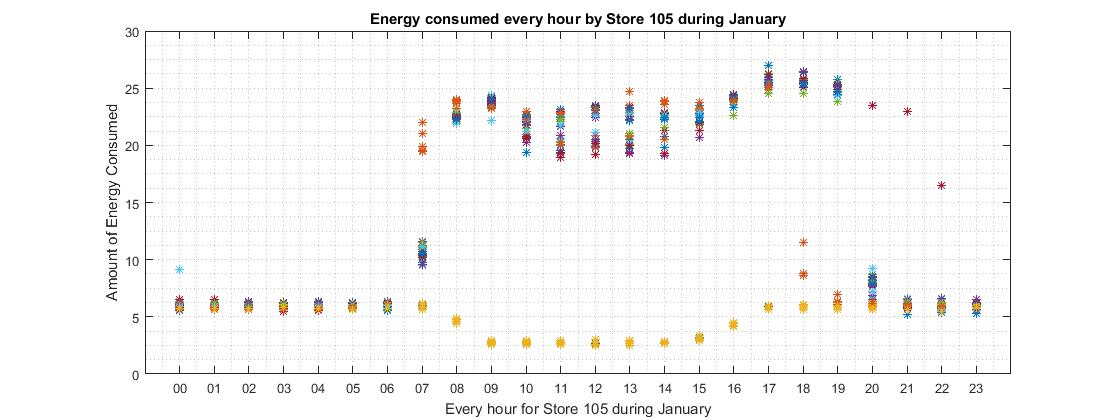
\includegraphics[scale=0.37]{new_105_jan_alldays.jpg}\label{102blockdiag}
	}
	\caption[The Block Diagram of the designed application]{Energy Consumption by Store 105 during January}
	\label{102blockdiag}
	\hspace{0cm}%
\end{figure}

As working days and non-working are mixed in this plot, therefore, it shall make sense if we treat them separately as energy consumption during the working days differs greatly from that during the non-working days. Analysis of this scatter plot led us to the induction of hour of the day in the feature vector as there is an increased energy consumption during working hours as compared to non-working hours.

\paragraph{} Now, in order for further analyze the power consumption we have to treat working days and non-working days differently. Therefore, we isolate the working days and non-working days from the Figure \ref{102blockdiag}, which are shown in Figure \ref{103blockdiag} and Figure \ref{104blockdiag}. 

\begin{figure}[H]
	\centering
	{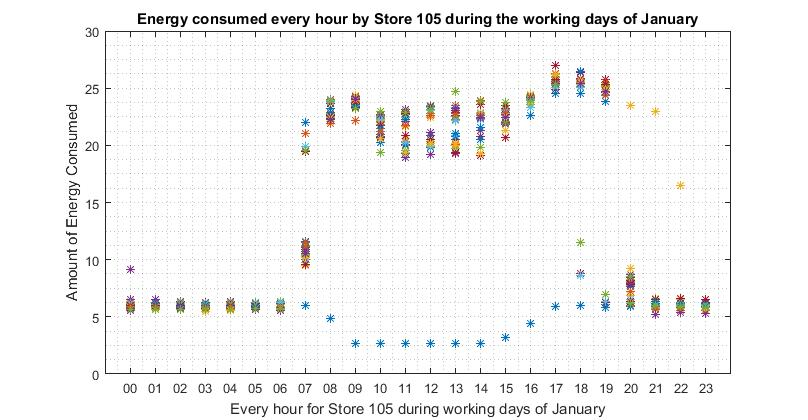
\includegraphics[scale=0.43]{new_105_jan_workdays.jpg}\label{103blockdiag}
	}
	\caption[The Block Diagram of the designed application]{Energy Consumption by Store 105 during the working days of January}
	\label{103blockdiag}
	\hspace{0cm}%
\end{figure}

Figure \ref{103blockdiag} provides a detailed insight of the operation of Store 105 during the working days as it shows that it opens up at around 7 am and remains opened till 7-8 pm in the evening. 

\begin{figure}[H]
	\centering
	{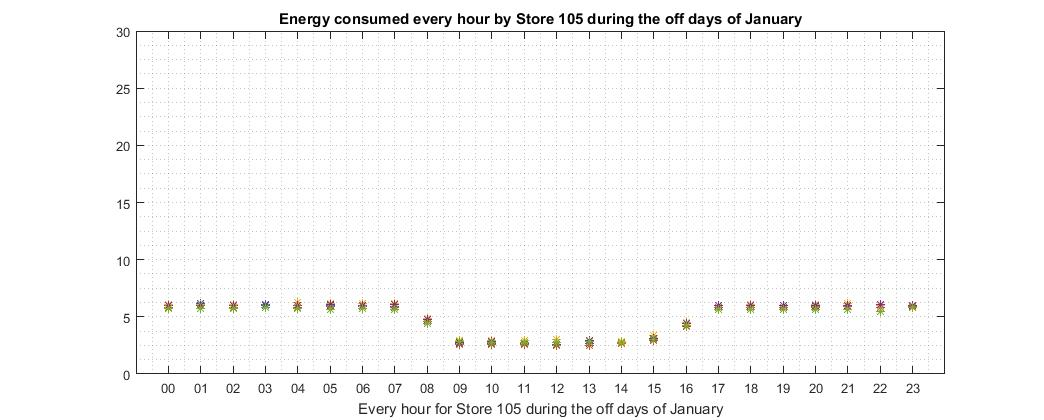
\includegraphics[scale=0.35]{new_105_jan_off_days1.jpg}\label{104blockdiag}
	}
	\caption[The Block Diagram of the designed application]{Energy Consumption by Store 105 during the off days of January}
	\label{104blockdiag}
	\hspace{0cm}%
\end{figure}

Whereas, during the non-working days, energy consumption remain relatively constant expect it is slightly lower during the day times possibly due to daylight (during the day, lighting and heating equipment might consume lower amount of energy).
\paragraph{}In order to select meaningful features to be implemented Machine Learning or Statistical Modeling, it is necessary to analyze the given data thoroughly.  After the analysis based on the previous plots, it was decided that the amount of energy consumption depends upon multiple factors, which are the store itself as all stores differs from one another as each having its particular size, different opening and closing hours, different number of energy consuming equipment and even have different geographical locations which affect the amount of energy consumption. Aside from that, time of the day is another factor as during working hours energy consumption is higher as shown in Figure \ref{103blockdiag} there is also a reduction in power consumption during the day even when the store is closed as shown in Figure \ref{104blockdiag}. It was also noticed from Figure \ref{100blockdiag} that energy consumption is slightly low during the summers, therefore, months also play a minor factor in the variation of energy consumption. As the stores do not operate during the Sundays and other public holidays as shown in Figure \ref{0blockdiag}, therefore, they are considered.

\paragraph{} Using this information, a Feature Vector (FV) $\in \mathbb{Re}^5 $ was made which is as follows,

Feature Vector (FV) = [Hour of the day, Store Number, Energy Consumed,Month, Tag for Working Day or Non-Working Day].





\paragraph{} 


%store number , hour, month, weekend or working day, 



\section{Methodologies}

Overall, the process consisted of two main steps which are as shown in Figure \ref{5blockdiag}, in which we obtain 5-dimensional  training input of size $m$ from Feature Vector which consists of energy consumption data, store number, number of month, hour of the day and tag for whether it is a working day or not. This data is analyzed and filtered of any potential outliers (k) as outliers generally serve to increase error in variance and lessen the capabilities of statistical tests. Therefore, Outlier Removal Algorithm was designed and implemented for that purpose, which is discussed in Section \ref{Outliers}.
\paragraph{} After the removal of outliers, we obtained data consisting of m-k examples as outliers (k) has been removed from the training dataset. Those m-k examples are then fed into the anomaly detection algorithm, which is discussed in Section \ref{anomalies}, which decides whether the given test input is anomalous or not as its output is in binary.

\begin{figure}[H]
	\centering
	{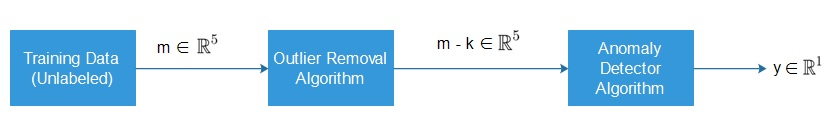
\includegraphics[scale=0.60]{block_anomaly.jpg}\label{5blockdiag}
	}
	\caption[The Block Diagram of the designed application]{The block diagram of anomaly detection algorithm where, \newline
	m = set of input training data \newline
    k = outliers \newline
    y = output.}
	\label{5blockdiag}
	\hspace{0.7cm}%
\end{figure}



\subsection{Outlier Removal Algorithm}
\label{Outliers}
In order to detect and remove outliers in the provided data, Tuckey's test was performed on the elements of feature vector, which involves the calculation of median of training data which is referred to $Q2$ and then again median of values lesser and greater than that of $Q2$ is calculated. Median of values lower than $Q2$ is refereed as $Q1$ (lower quartile) and those having greater than $Q2$ is referred as $Q3$ (upper quartile) as shown in Figure \ref{4blockdiag}.
\paragraph{} After determining $Q1$ and $Q3$, then Interquartile range is calculated by subtracting the value at $Q3$ by $Q1$.
\begin{equation}
IQR = Q3-Q1
\end{equation}

After calculating the Interquartile Range (IQR), we use it to calculate the Tuckey's Fences or Inner Fences by the following equation,

\begin{equation}
Inner Fence Lower Limit = Q1 - \alpha(IQR)
\end{equation}
\begin{equation}
Inner Fence Upper Limit = Q3 + \alpha(IQR)
\end{equation}
       where, \newline $\mathbf{\alpha}$ is the hyperparameter which varies the inner fence limits.

\begin{figure}[H]
	\centering
	{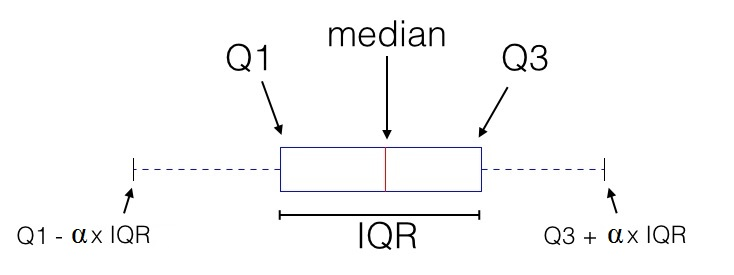
\includegraphics[scale=0.60]{quartiles.jpg}\label{4blockdiag}
	}
	\caption[The Block Diagram of the designed application]{Depiction of quartiles as used in the detection and removal of Outliers}
	\label{4blockdiag}
	\hspace{0.7cm}%
\end{figure}



Any value lying beyond inner fence limits (upper and lower) can be considered as an outlier, and therefore, it is removed. A sample result of designed outlier detection algorithm is shown in Figure \ref{7QRX4}.






\subsection{Anomaly Detection Algorithm}
\label{anomalies}
In order to test the energy consumption anomalies, the output of Outlier Removal Algorithm which consisted of set of training data without outliers (m-k) examples are fed to the anomaly detector. The input contains the same information as 5-dimensional feature vector about the amount of energy consumed,hour of the day, store number, month and whether it is a working day or not as well as learning parameter $\beta$.

\paragraph{} The learning parameter $\beta$ is used to give equivalent amount of standard deviation as its value to the value of energy consumption. For example, if $\beta$ = 2, then we can consider energy data which is $2\sigma$ away from the mean as shown in Figure \ref{blockdiag} as not an anomaly. The lower the value of $\beta$ the higher the chance of getting the test input as an anomaly and vice versa. 
\begin{equation}
\label{equation_anomaly}
\mu-\beta\sigma \leq x \leq \mu + \beta\sigma
\end{equation}
where, \newline $\mu$ is mean \newline
$x$ is test input \newline
$\sigma$ is standard deviation \newline
$\beta$ is the learning parameter

\paragraph{}If the test input $x$ lies within the constraints of this equation then it is considered as not an anomaly, otherwise it is considered as an anomaly or in other words, output $y \in \mathbb{Re}^1$, where $\mathbb{Re}^1$ = \{0,1\}, where 0 represents not an anomaly and 1 represents an anomaly in the test input.

\begin{figure}[H]
	\centering
	{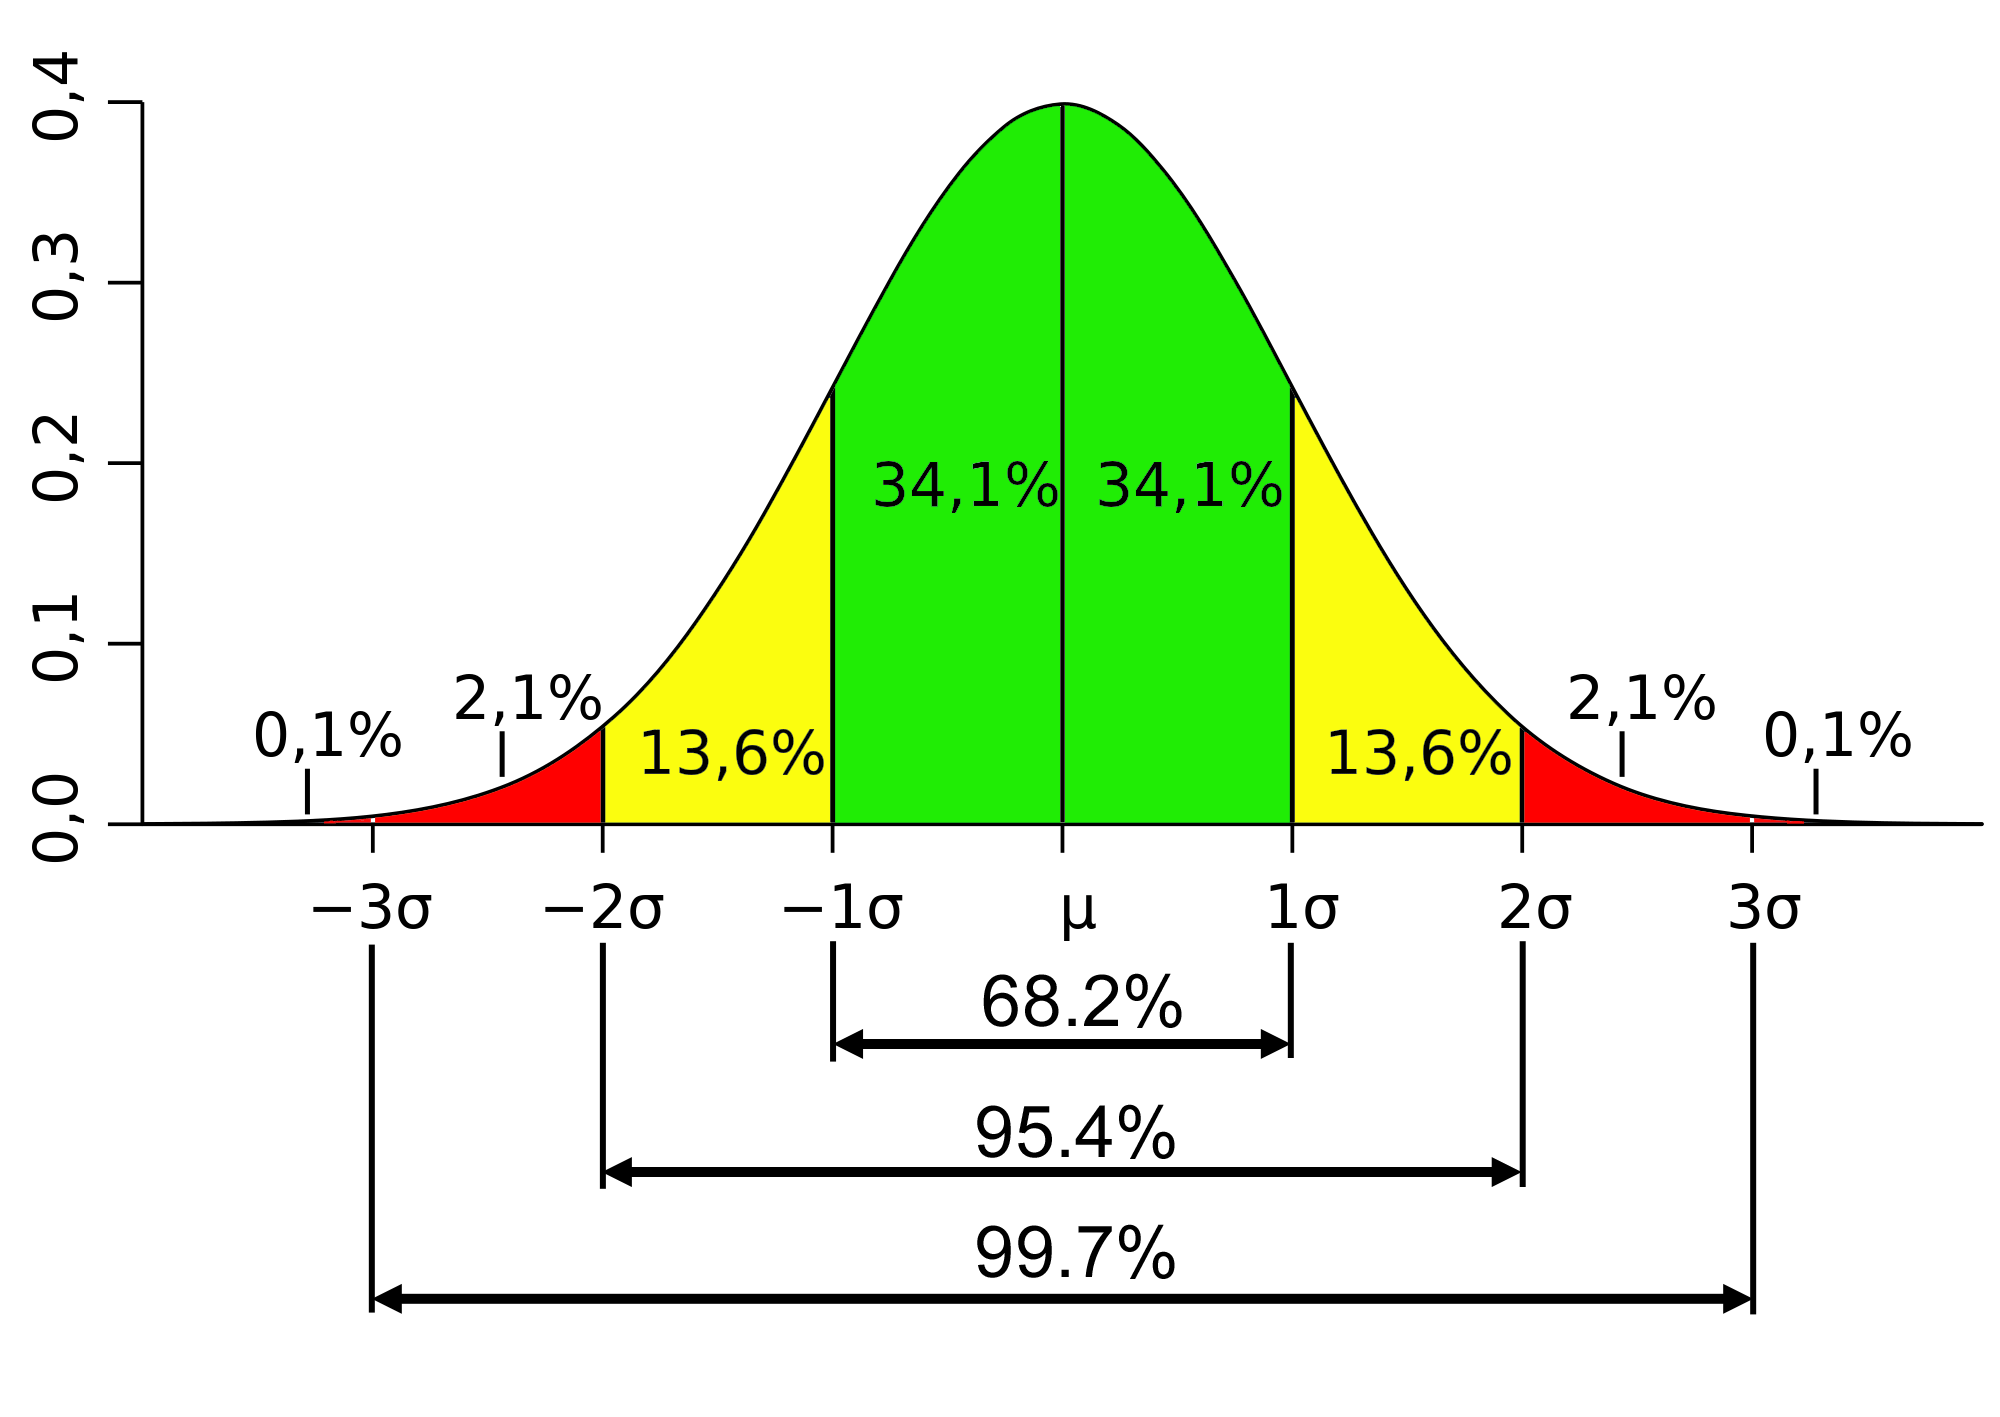
\includegraphics[scale=0.15]{Gaussian_bell.png}\label{blockdiag}
	}
	\caption[The Block Diagram of the designed application]{The learning rate $\beta$ corresponds to the standard deviation $\sigma$ of this Gaussian plot}
	\label{blockdiag}
	\hspace{0.7cm}%
\end{figure}

%\section{Methods of Univariate Outlier Detection}




%\section{Test Data and Feature Vector}
%\label{Test Data and Feature Vector}


\section{Test Results}\label{Test Results}
In this section, the overall results are discussed as to how well the outlier and anomaly detection algorithms performed when test inputs were given to them.


\subsection{Performance of Outlier Detection Algorithm}

Outlier detection algorithm was developed and it performed adequately in removing outliers. Figure \ref{7blockdiag} shows the energy consumption data of each hour for all working days in January 2016 for a particular store, whereas, Figure \ref{7QRX4} shows the same data as in Figure \ref{7blockdiag} after the outlier removal algorithm implemented on it.

\subsubsection{Implementation of Outlier Detection Algorithm on Working Days}

As discussed in section \ref{Data}, among all of the factors, the main difference in the amount of energy consumption was observed between working days and non-working days especially during the usual working hours of the stores. Therefore, those days are treated separately. The following plots illustrate performance of Outlier Detection Algorithm on a sample data of Store 105 during the working days of January 2016. Figure \ref{7blockdiag} shows the energy consumption data of the corresponding with outliers present in it. Whereas, Figure \ref{7QRX4} and Figure \ref{7QRX5} represent the same test input with Outlier Detection Algorithm implemented on it with $\alpha$ = 1.5 and 0.9 respectively.

\begin{figure}[H]
	\centering
	{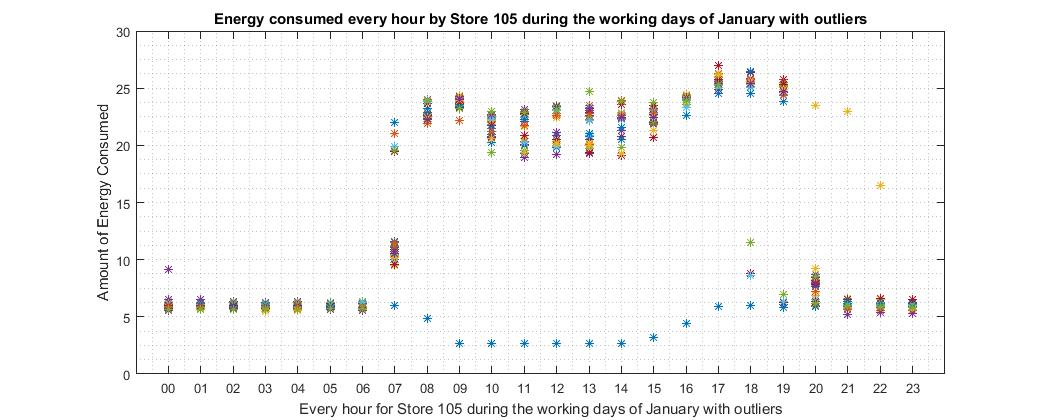
\includegraphics[scale=0.40]{105_ol_new_last.jpg}\label{7blockdiag}
	}
	\caption[The Block Diagram of the designed application]{Energy Consumption by Store 105 during working days of January 2016 with outliers present}
	\label{7blockdiag}
	\hspace{0.7cm}%
\end{figure}

\begin{figure}[H]
	\centering
	{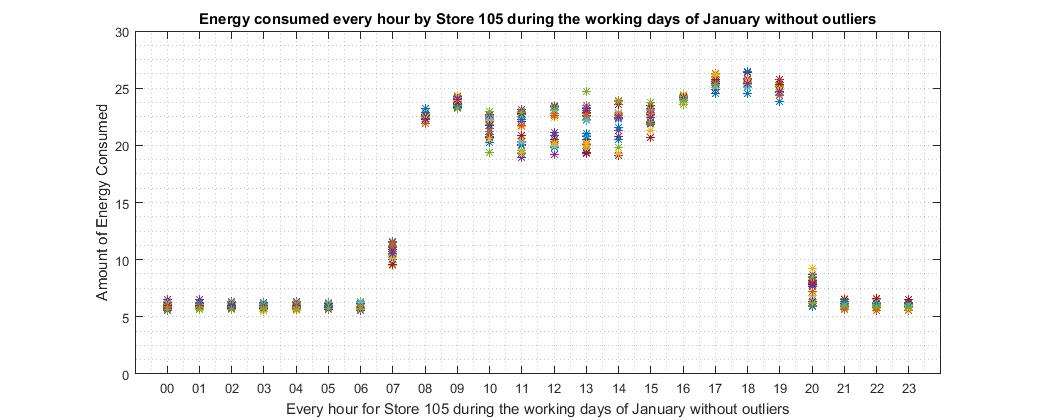
\includegraphics[scale=0.40]{alpha_15.jpg}\label{7QRX4}
	}
	\caption[Energy Consumption during the month of January by store 105 (same dataset as in Figure \ref{7blockdiag}) without outliers]{Energy Consumption during the month of January by store 105 without outliers with $\alpha$ = 1.5}
	\label{7QRX4}
	\hspace{1cm}%
\end{figure}
\paragraph{}Figure \ref{7QRX4} illustrates the same test input as in Figure \ref{7blockdiag} with outliers removed from it. The hyperparameter $\alpha$ which determine the fence limit in Tuckey's test as explained in section \ref{Outliers} was set to be equal to 1.5 in that case. 
\paragraph{} The Table \ref{table:studies3} shows how many values of energies were considered anomalous and were removed by outlier detection algorithm which were to be around 7\% of all test energy values if $\alpha$ = 1.5.


\begin{table}[H]
	\centering
	{\renewcommand{\arraystretch}{1.0} 
		\begin{tabular}{|c|c|c|}
			\hline %\toprule
			%\multicolumn{2}{c}{studies}\\ \cmidrule{1-2}
			Hour of the Day & Total Working days (m) & Number of Outliers(k)\\
			\hline	%\midrule
			00 & 25 &1
			\\ \hline  %\addlinespace
			01 & 25 & 0 \\ \hline %\addlinespace
			02 & 25 & 0\\  \hline  %\addlinespace
			03 & 25 &0\\ 
			\hline	%\bottomrule
			04 & 25 & 0 \\ \hline  %\addlinespace
			05 & 25 & 0 \\ \hline %\addlinespace
			06 & 25 & 0\\  \hline  %\addlinespace
			07 & 25 &6 \\ 
			\hline	%\bottomrule
			08 & 25 &5 \\ 
			\hline	%\bottomrule
			09 & 25 & 2 \\ \hline  %\addlinespace
			10 &25 & 1\\ \hline %\addlinespace
			11 & 25 &1 \\  \hline  %\addlinespace
			12 & 25 &1 \\ 
			\hline	%\bottomrule
			13 &25 & 1 \\ \hline %\addlinespace
			14 & 25 &1 \\  \hline  %\addlinespace
			15 & 25 &1\\ 
			\hline	%\bottomrule
			16 &25 & 3 \\ \hline %\addlinespace
			17 & 25 & 2\\  \hline  %\addlinespace
			18 & 25 &6 \\ \hline
			19 & 25 & 6 \\ \hline %\addlinespace
			20 & 25  & 1\\  \hline  %\addlinespace
			21 & 25 &2 \\ 
			\hline	%\bottomrule
			22 &25 & 2 \\ \hline %\addlinespace
			23 & 25 & 2\\  \hline  %\addlinespace
		\end{tabular}
	}
	\caption{Number of working days having Outliers in January 2016 for Store 105 when $\alpha$ = 1.5}.
	\label{table:studies3}
\end{table}



\begin{figure}[H]
	\centering
	{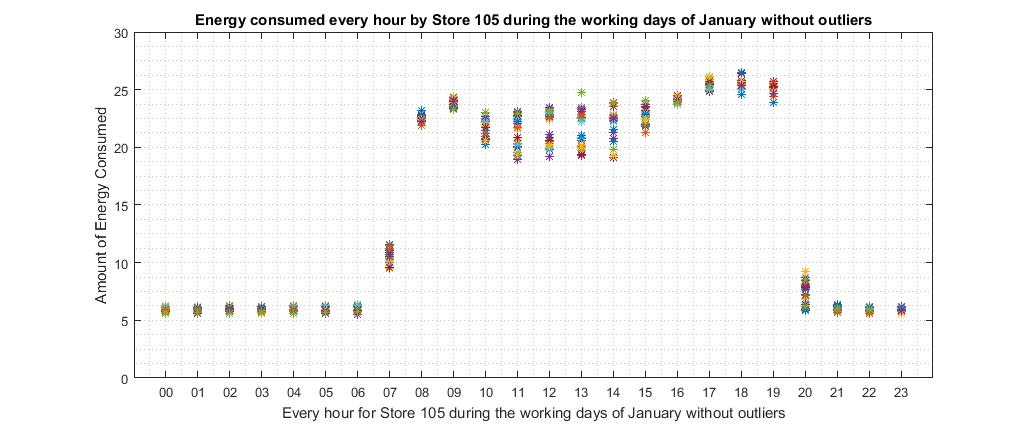
\includegraphics[scale=0.40]{105_nol_new_last.jpg}\label{7QRX5}
	}
	\caption[Energy Consumption during the month of January by store 105 (same dataset as in Figure \ref{7blockdiag}) without outliers]{Energy Consumption during the month of January by store 105 without outliers with $\alpha$ = 0.9}
	\label{7QRX5}
	\hspace{1cm}%
\end{figure}

\paragraph{} In case of Figure \ref{7QRX5} hyperparameter $\alpha$  was set to be equal to 0.9. The Table \ref{table:studies2} shows how many values of energies were considered anomalous and were removed by outlier detection algorithm which were to be around 9.5\% of all test energy values if $\alpha$ = 0.9. 
\begin{table}[H]
	\centering
	{\renewcommand{\arraystretch}{1.0} 
		\begin{tabular}{|c|c|c|}
			\hline %\toprule
			%\multicolumn{2}{c}{studies}\\ \cmidrule{1-2}
			Hour of the Day & Total Working days (m) & Number of Outliers(k)\\
			\hline	%\midrule
			00 & 25 &4
			\\ \hline  %\addlinespace
			01 & 25 & 1 \\ \hline %\addlinespace
			02 & 25 & 1\\  \hline  %\addlinespace
			03 & 25 &1 \\ 
			\hline	%\bottomrule
			04 & 25 & 0 \\ \hline  %\addlinespace
			05 & 25 & 0 \\ \hline %\addlinespace
			06 & 25 & 2\\  \hline  %\addlinespace
			07 & 25 &6 \\ 
			\hline	%\bottomrule
			08 & 25 &5 \\ 
			\hline	%\bottomrule
			09 & 25 & 2 \\ \hline  %\addlinespace
			10 &25 & 2\\ \hline %\addlinespace
			11 & 25 &1 \\  \hline  %\addlinespace
			12 & 25 &1 \\ 
			\hline	%\bottomrule
			13 &25 & 1 \\ \hline %\addlinespace
			14 & 25 &1 \\  \hline  %\addlinespace
			15 & 25 &1\\ 
			\hline	%\bottomrule
			16 &25 & 5 \\ \hline %\addlinespace
			17 & 25 & 4\\  \hline  %\addlinespace
			18 & 25 &6 \\ \hline
			19 & 25 & 6 \\ \hline %\addlinespace
			20 & 25  & 1\\  \hline  %\addlinespace
			21 & 25 &4 \\ 
			\hline	%\bottomrule
			22 &25 & 4 \\ \hline %\addlinespace
			23 & 25 & 4\\  \hline  %\addlinespace
		\end{tabular}
	}
	\caption{Number of working days having Outliers in January 2016 for Store 105 when $\alpha$ = 0.9}.
	\label{table:studies2}
\end{table}



\paragraph{}If we compare both Figure \ref{7QRX4} and Figure \ref{7QRX5}, we can see that both removed apparent outliers, except that in Figure \ref{7QRX5}, the limits of inner fence were smaller, therefore, it removed outliers more strictly (around 7\% and 9.5\% in case of $\alpha$ =1.5 and 0.9 respectively) and may be some normal distribution values also got removed with them as well. Therefore, the value of $\alpha$ should be tuned accordingly if labeled data is provided. 

\subsubsection{Implementation of Outlier Algorithm on Non-working Days}
Similarly like working days in previous plots, the Outlier Detection Algorithm was implemented on the energy consumption data of non-working days. The following plots illustrate the performance of that. Figure \ref{8QRX5} shows the unfiltered data, whereas Figure \ref{9QRX5} shows the same data of energy consumption with Outlier Detection Algorithm implemented on it.

\begin{figure}[H]
	\centering
	{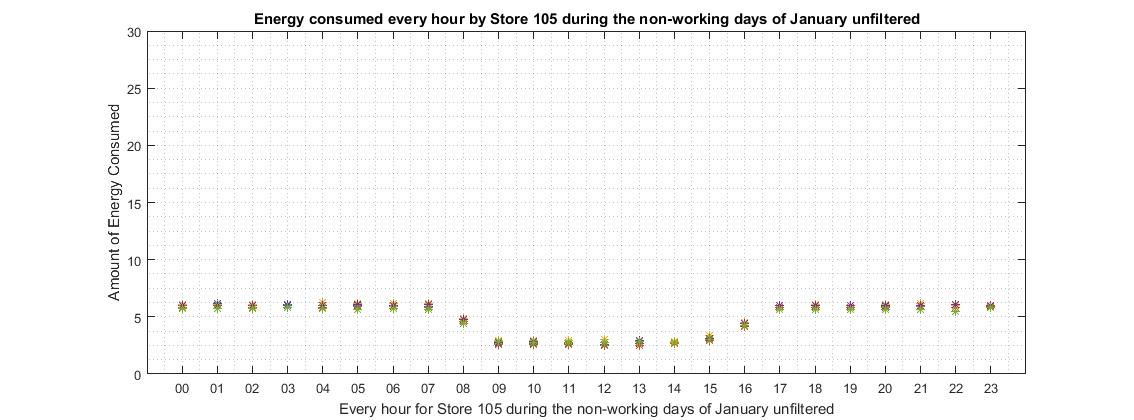
\includegraphics[scale=0.32]{alpha_15_unfiltered_off.jpg}\label{8QRX5}
	}
	\caption[Energy Consumption during the month of January by store 105 (same dataset as in Figure \ref{7blockdiag}) without outliers]{Energy Consumption for non-working days during the month of January by store 105 without Outlier Detection Algorithm}
	\label{8QRX5}
	\hspace{0.1cm}%
\end{figure}

\begin{figure}[H]
	\centering
	{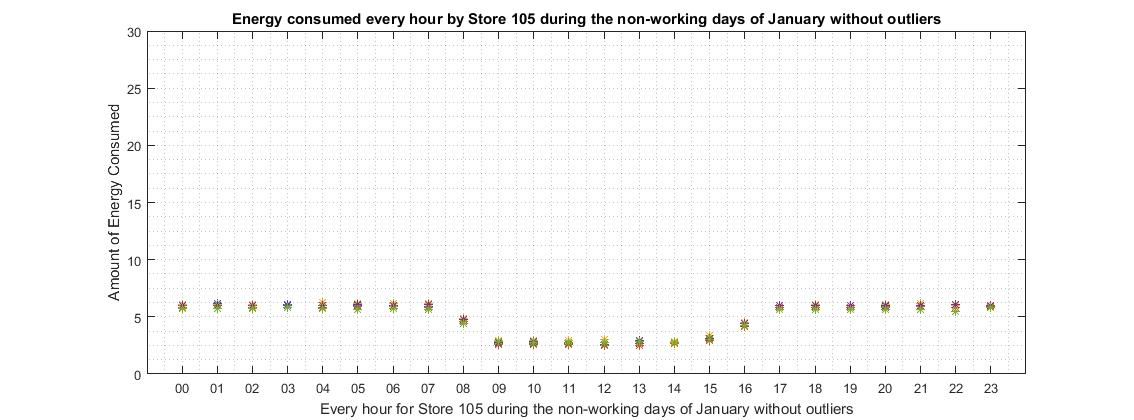
\includegraphics[scale=0.32]{alpha_15_nol_off.jpg}\label{9QRX5}
	}
	\caption[Energy Consumption during the month of January by store 105 (same dataset as in Figure \ref{7blockdiag}) without outliers]{Energy Consumption for non-working days during the month of January by store 105 with Outlier Detection Algorithm with $\alpha$ = 0.9}
	\label{9QRX5}
	\hspace{0.1cm}%
\end{figure}

As it is obvious that Figure \ref{8QRX5} and \ref{9QRX5} are identical as there were no outliers in the energy consumption data as it shows repetitive pattern and is quite compact for all 5 non-working days. Therefore, due to that reason, Outlier Detection algorithm hasn't removed anything since there are no anomalous energy consumption values present.


\subsection{Performance of Anomaly Detection Algorithm}

After the removal of outliers , and for Anomaly Detection algorithm, mean($\mu$) and standard deviation ($\sigma$) of each hour of the day is calculated and in order to decide whether, certain example is an anomaly or not, the hyperparameter $\beta$ has to be tuned.

\paragraph{} The following tables show the 24 different models for each hour of the day for a particular store for a certain month, since working days and non-working days are treated separately, therefore, we obtained 48 different models in 2 separate tables each for working day and non-working day. Every model contains the mean($\mu$) and standard deviation($\sigma$) of a particular hour of the day for all the working days or non-working days of the corresponding month.
\paragraph{} These values are used by Anomaly detection algorithm in equation \ref{equation_anomaly} to decide whether our test input is anomalous or not. If the value of our test input lies within the constraints of that equation, then it is considered as non-anomalous, otherwise it is considered an anomaly in power consumption.

\paragraph{} In table \ref{table:studies}, the mean($\mu$) and standard deviation($\sigma$) for all 25 working days of January 2016 for store 105 is shown.  


\begin{table}[H]
	\centering
	{\renewcommand{\arraystretch}{1.0} 
		\begin{tabular}{|c|c|c|}
			\hline %\toprule
			%\multicolumn{2}{c}{studies}\\ \cmidrule{1-2}
			Hour of the Day & Mean($\mathbf{\mu}$) & Standard Deviation($\mathbf{\sigma}$)\\
			\hline	%\midrule
			00 & 5.942
			 & 0.1793
			  \\ \hline  %\addlinespace
			01 & 5.916 & 0.1760 \\ \hline %\addlinespace
			02 & 5.919 & 0.1853\\  \hline  %\addlinespace
			03 & 5.929 &0.1667 \\ 
			\hline	%\bottomrule
			04 & 5.904 & 0.1964 \\ \hline  %\addlinespace
			05 & 5.879 & 0.1936 \\ \hline %\addlinespace
			06 & 5.8673 & 0.2216\\  \hline  %\addlinespace
			07 & 10.6137 &0.6090 \\ 
			\hline	%\bottomrule
			08 & 22.4845 &0.2975 \\ 
			\hline	%\bottomrule
			09 & 23.7458 & 0.3356 \\ \hline  %\addlinespace
			10 &21.7864 & 0.7461\\ \hline %\addlinespace
			11 & 21.458 &1.3724 \\  \hline  %\addlinespace
			12 & 21.766 &1.4433 \\ 
			\hline	%\bottomrule
			13 &21.668 & 1.5485 \\ \hline %\addlinespace
			14 & 21.811 &1.4422 \\  \hline  %\addlinespace
			15 & 22.6104 & 0.7274\\ 
			\hline	%\bottomrule
			16 &24.1545 & 0.2071 \\ \hline %\addlinespace
			17 & 25.5056 & 0.3360\\  \hline  %\addlinespace
			18 & 25.5325 &0.4310 \\ \hline
			19 & 24.92 & 0.4770 \\ \hline %\addlinespace
			20 & 7.407  & 0.9895\\  \hline  %\addlinespace
			21 & 6.0273 &0.1806 \\ 
			\hline	%\bottomrule
			22 &5.9704 & 0.1753 \\ \hline %\addlinespace
			23 & 5.9647 & 0.1511\\  \hline  %\addlinespace
		\end{tabular}
}
\caption{Mean ($\mathbf{\mu}$) and Standard Deviation ($\mathbf{\sigma}$) of Power Consumption in Store 105 during the working days of January 2016}.
\label{table:studies}
\end{table}

\paragraph{} In table \ref{table:studies1}, the mean($\mu$) and standard deviation($\sigma$) for the remaining 6 non-working days of January 2016 for store 105 is shown. 

\begin{table}[H]
	\centering
	{\renewcommand{\arraystretch}{1.0} 
		\begin{tabular}{|c|c|c|}
			\hline %\toprule
			%\multicolumn{2}{c}{studies}\\ \cmidrule{1-2}
			Hour of the Day & Mean($\mathbf{\mu}$) & Standard Deviation($\mathbf{\sigma}$)\\
			\hline	%\midrule
			00 & 5.94 &0.1376 \\ \hline  %\addlinespace
			01 &5.94  & 0.1925 \\ \hline %\addlinespace
			02 &5.935  &0.1485 \\  \hline  %\addlinespace
			03 & 5.97 & 0.1350\\ \hline	%\bottomrule
			04 & 5.955 &0.2057  \\ \hline  %\addlinespace
			05 & 5.955 & 0.1979 \\ \hline %\addlinespace
			06 & 5.94 &0.1663 \\  \hline  %\addlinespace
			07 & 5.915 &0.1875\\ \hline	%\bottomrule
			08 & 4.67 &0.1735 \\ \hline	%\bottomrule
			09 & 2.74 & 0.1567 \\ \hline  %\addlinespace
			10 &2.75 &0.1211 \\ \hline %\addlinespace
			11 & 2.72 &0.1279 \\  \hline  %\addlinespace
			12 & 2.73 &0.2079 \\ \hline	%\bottomrule
			13 &2.74 &0.1825  \\ \hline %\addlinespace
			14 & 2.735 &0.0821 \\  \hline  %\addlinespace
			15 & 3.1 &0.15 \\ \hline	%\bottomrule
			16 &4.29 & 0.1442 \\ \hline %\addlinespace
			17 &5.85  &0.1468 \\  \hline  %\addlinespace
			18 & 5.895 &0.1726 \\ \hline
			19 &5.855  & 0.1652 \\ \hline %\addlinespace
			20 &5.905   &0.1832 \\  \hline  %\addlinespace
			21 & 5.915 &0.1957 \\ \hline	%\bottomrule
			22 &5.86 &0.2219  \\ \hline %\addlinespace
			23 &5.925  &0.0918 \\  \hline  %\addlinespace
		\end{tabular}
	}
	\caption{Mean ($\mathbf{\mu}$) and Standard Deviation ($\mathbf{\sigma}$) of Power Consumption in Store 105 during the off days of January 2016}.
	\label{table:studies1}
\end{table}

\section{Outlook}
\label{Outlook}
In this project, the energy consumption data which was provided by the Tengelmann Group was analyzed to extract meaningful features and anomaly detection algorithm was developed and implemented by using that provided data. In order to do so, the data was analyzed and in that analysis, several factors were identified which affected the energy consumption which were the corresponding month, difference in energy consumption during working day and non-working day, hour of the day. Therefore, a feature vector was made consisting of information about month, store number, energy consumption,hour of the day and binary tag for working and non-working day which is discussed in section \ref{Data}.
\paragraph{} Afterward,  this feature vector was fed to the Outlier detection algorithm in order to remove any superfluous energy consumption values from it as discussed in section \ref{Outliers} and the values without outliers were analyzed for anomalies in Anomaly detection algorithm discussed in section \ref{anomalies}.

\paragraph{} The obtained results from those algorithm are visualized and discussed in section \ref{Test Results}, which can be cross validated if some labeled data is provided.




%\bibliographystyle{abbrv}
%\bibliography{simple}

%Questions to ask
%why standard deviation and tukey's algorithm both used in outlier detection?
%should I mention the limitations of univariate outlier detection method?
%what is Beta and how does it affect?
%the variable multiple for inner fence should be used as an input?
%which pictures should I put? may be scatter plots?? how many??
%problem description part?


\end{document}
This is never printed
